\section{Volume}

\subsection{Volume: Given cross-sectional shapes}
The below picture is given as an example. This object's base is defined by it's cross-sections which are squares who's length is defined by a graph's height.

\begin{figure}[H]
	\begin{center}
		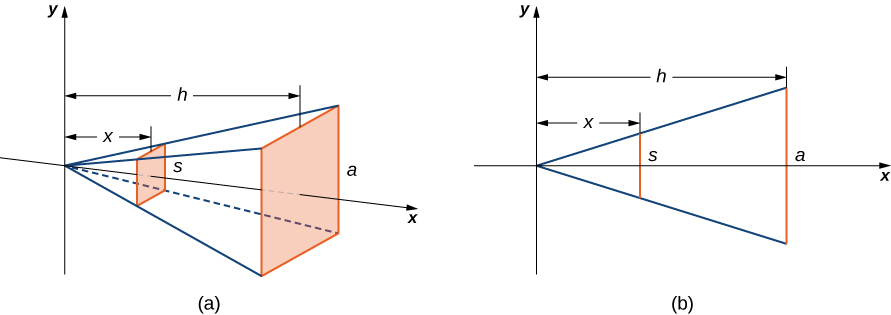
\includegraphics[scale=0.50]{pages/images/crossbase}
		\label{fig:fig4}
	\end{center}
\end{figure}

The idea with these problems is that we have to find the area function, once we find the area function we can apply that to our integral with the bounds given. The simple formula is:

\begin{equation}
	V = \int_a^b{A(x)} dx
\end{equation}

\pagebreak
\subsection{Rotational Volume: Washer Method}
Volume by washer is the easlist to visualize, circular disks are formed by the areas from heights of the two functions. We know the area function is defined by 

\begin{align*}
	A &= \pi r^2 \\ 
	A &= \pi (f(x))^2
\end{align*}

Now let's consider, $g(x)$, where $g(x) \leq f(x)$, on the interval $[a,b]$. 
\begin{align*}
	A &= \pi f(x)^2 - \pi g(x)^2 = \pi(f(x)^2 - g(x)^2)
\end{align*}

Now let's put into integral form:

\begin{equation}
	V = \pi\int_a^b{f(x)^2-g(x)^2} dx
\end{equation}

Now if we revolved around another axis, we need to find the distance from the functions to that axis, if $\phi$ is the axis which is less then $f,g$: 

\begin{equation}
	V = \pi\int_a^b{(f(x)-\phi)^2-(g(x)-\phi)^2}dx
\end{equation}


\begin{figure}[H]
	\begin{center}
		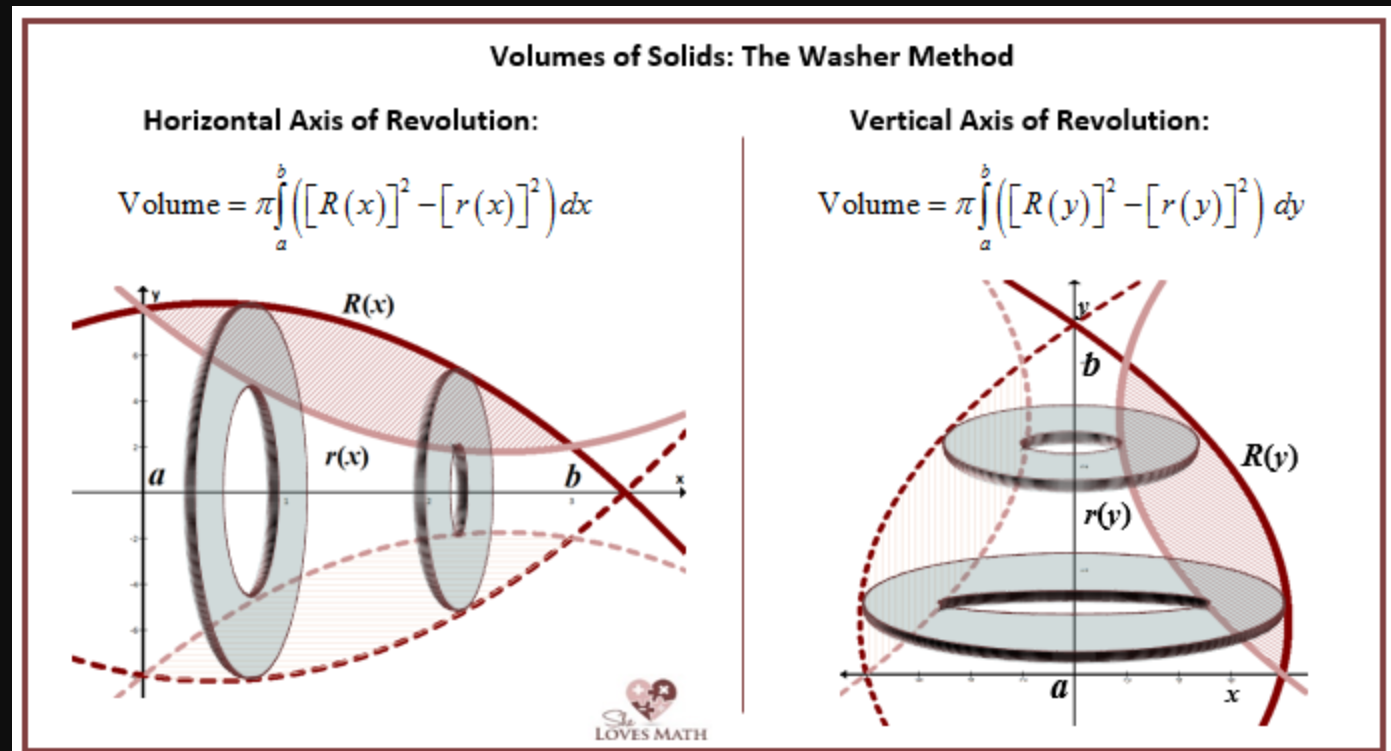
\includegraphics[scale=0.30]{pages/images/washers}
		\label{fig:fig4}
	\end{center}
\end{figure}

\pagebreak

\subsection{Rotational Volume: Shell Method}
Volume by shell is another method of gathering a rotational volume when you are presented with a different axis of rotation. While the washer method is much more easier for many problems, when rotating around the y-axis with a function that can't be easily set in terms of y, volume by shell is a better way to go.

\begin{figure}[H]
	\begin{center}
		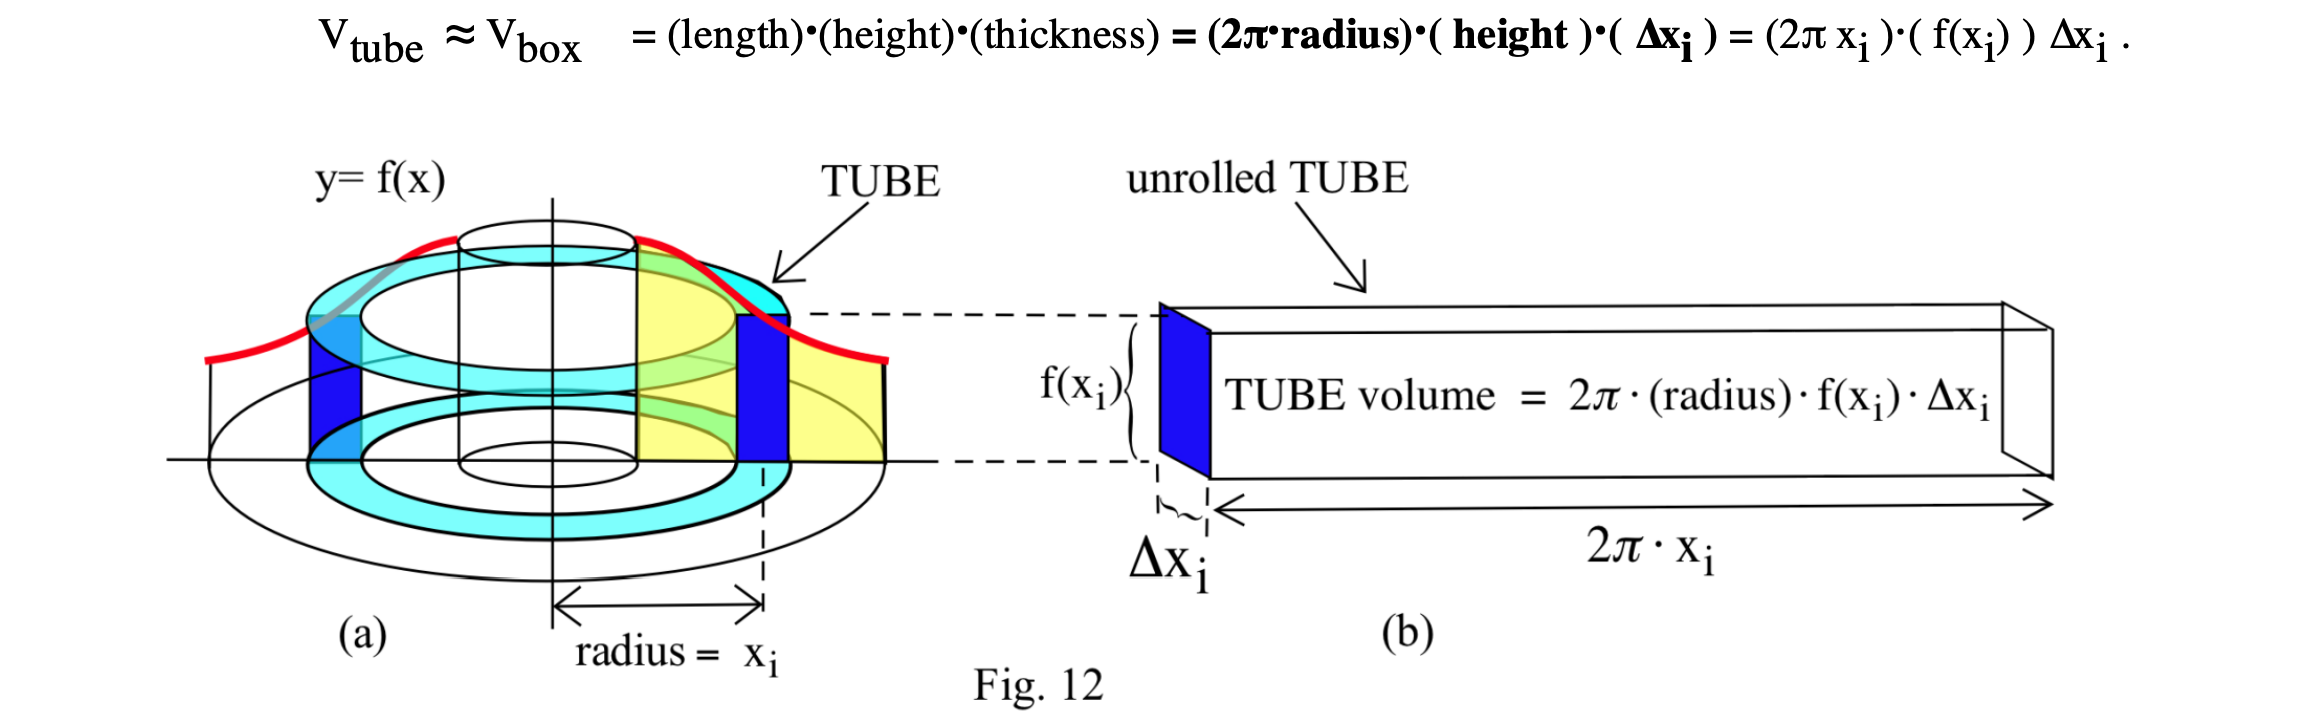
\includegraphics[scale=0.30]{pages/images/vshell}
		\label{fig:fig3}
	\end{center}
\end{figure}

We can now write the formula for volume now: 

\begin{equation}
	V = lwh 
\end{equation}
\begin{equation}
	V = 2\pi x_i f(x) \Delta x 
\end{equation}

Now the integral form, given $f=f(x)$, and $g = g(x)$, where $f\geq g$, on the 
interval $[a, b]$
\begin{equation}
	V = 2\pi \int_a^b{x(f-g)}dx
\end{equation}